%# -*- coding: utf-8-unix -*-
%%==================================================
%% chapter01.tex for SJTU Master Thesis
%%==================================================

%\bibliographystyle{sjtu2}%[此处用于每章都生产参考文献]
\chapter{AKI算法}
\label{chap:Alg}

为了确定一个子密钥集合$K$的实际密钥信息,我们需要一个算法来计算AKI的值并得到一些可能的实际密钥信息集合。
黄佳琳博士在其博士论文\cite{huang2014revisiting}中提出了一个自动化搜索密钥信息泄露的工具,但该工具设计的算法是一个贪心算法,只能计算出AKI的一个合理上界,无法得到真实的AKI值。
一个AKI的合理上界可以用来进行攻击可能性的分析,但无法用来实际分析一个密钥编排方案的强弱。
Lin等人在\citen{lin2016automatic}中提出了一种对密钥桥技术(Key-Bridging Technique\citen{dunkelman2010improved})的自动化搜索算法,但时间复杂度极高,无法进行大量不同$K$的计算,并且也存在一些反例无法计算(后文中将会提到一个反例)。
因此,现有的AKI算法由于只能给出AKI的一个合理上界,只能用于攻击分析,无法用来分析密钥编排方案的强弱好坏,也不能用来改进密钥编排方案的设计。
本章将会介绍一种全新的基于图论的AKI算法,将会在多项式时间复杂度内计算出真实的AKI值。

\section{单轮加密的AKI}
在介绍完整的AKI算法之前,我们首先从简化版的问题开始考虑——仅有一轮加密时的AKI计算。
我们假设子密钥集合$K$全部集中在第$r$轮上,然后只考虑$r$轮和$r-1$轮两轮之间的依赖关系。
为了解决这个问题,我们将使用图论中二分图的思想来将编排方案、密钥比特、依赖关系等参数量化成图,进而将AKI的计算转化为一个图论的问题。
\begin{defn}[二分图]
    设$G(V,E)$是一个无向图,如果顶点集合$V$可以分割为两个互不相交的子集$A,B$且图中每条边的两个顶点分别属于不同的子集,则称$G$为一个二分图,可记为$G(A,B,E)$。
\end{defn}
\begin{figure}
    \centering
    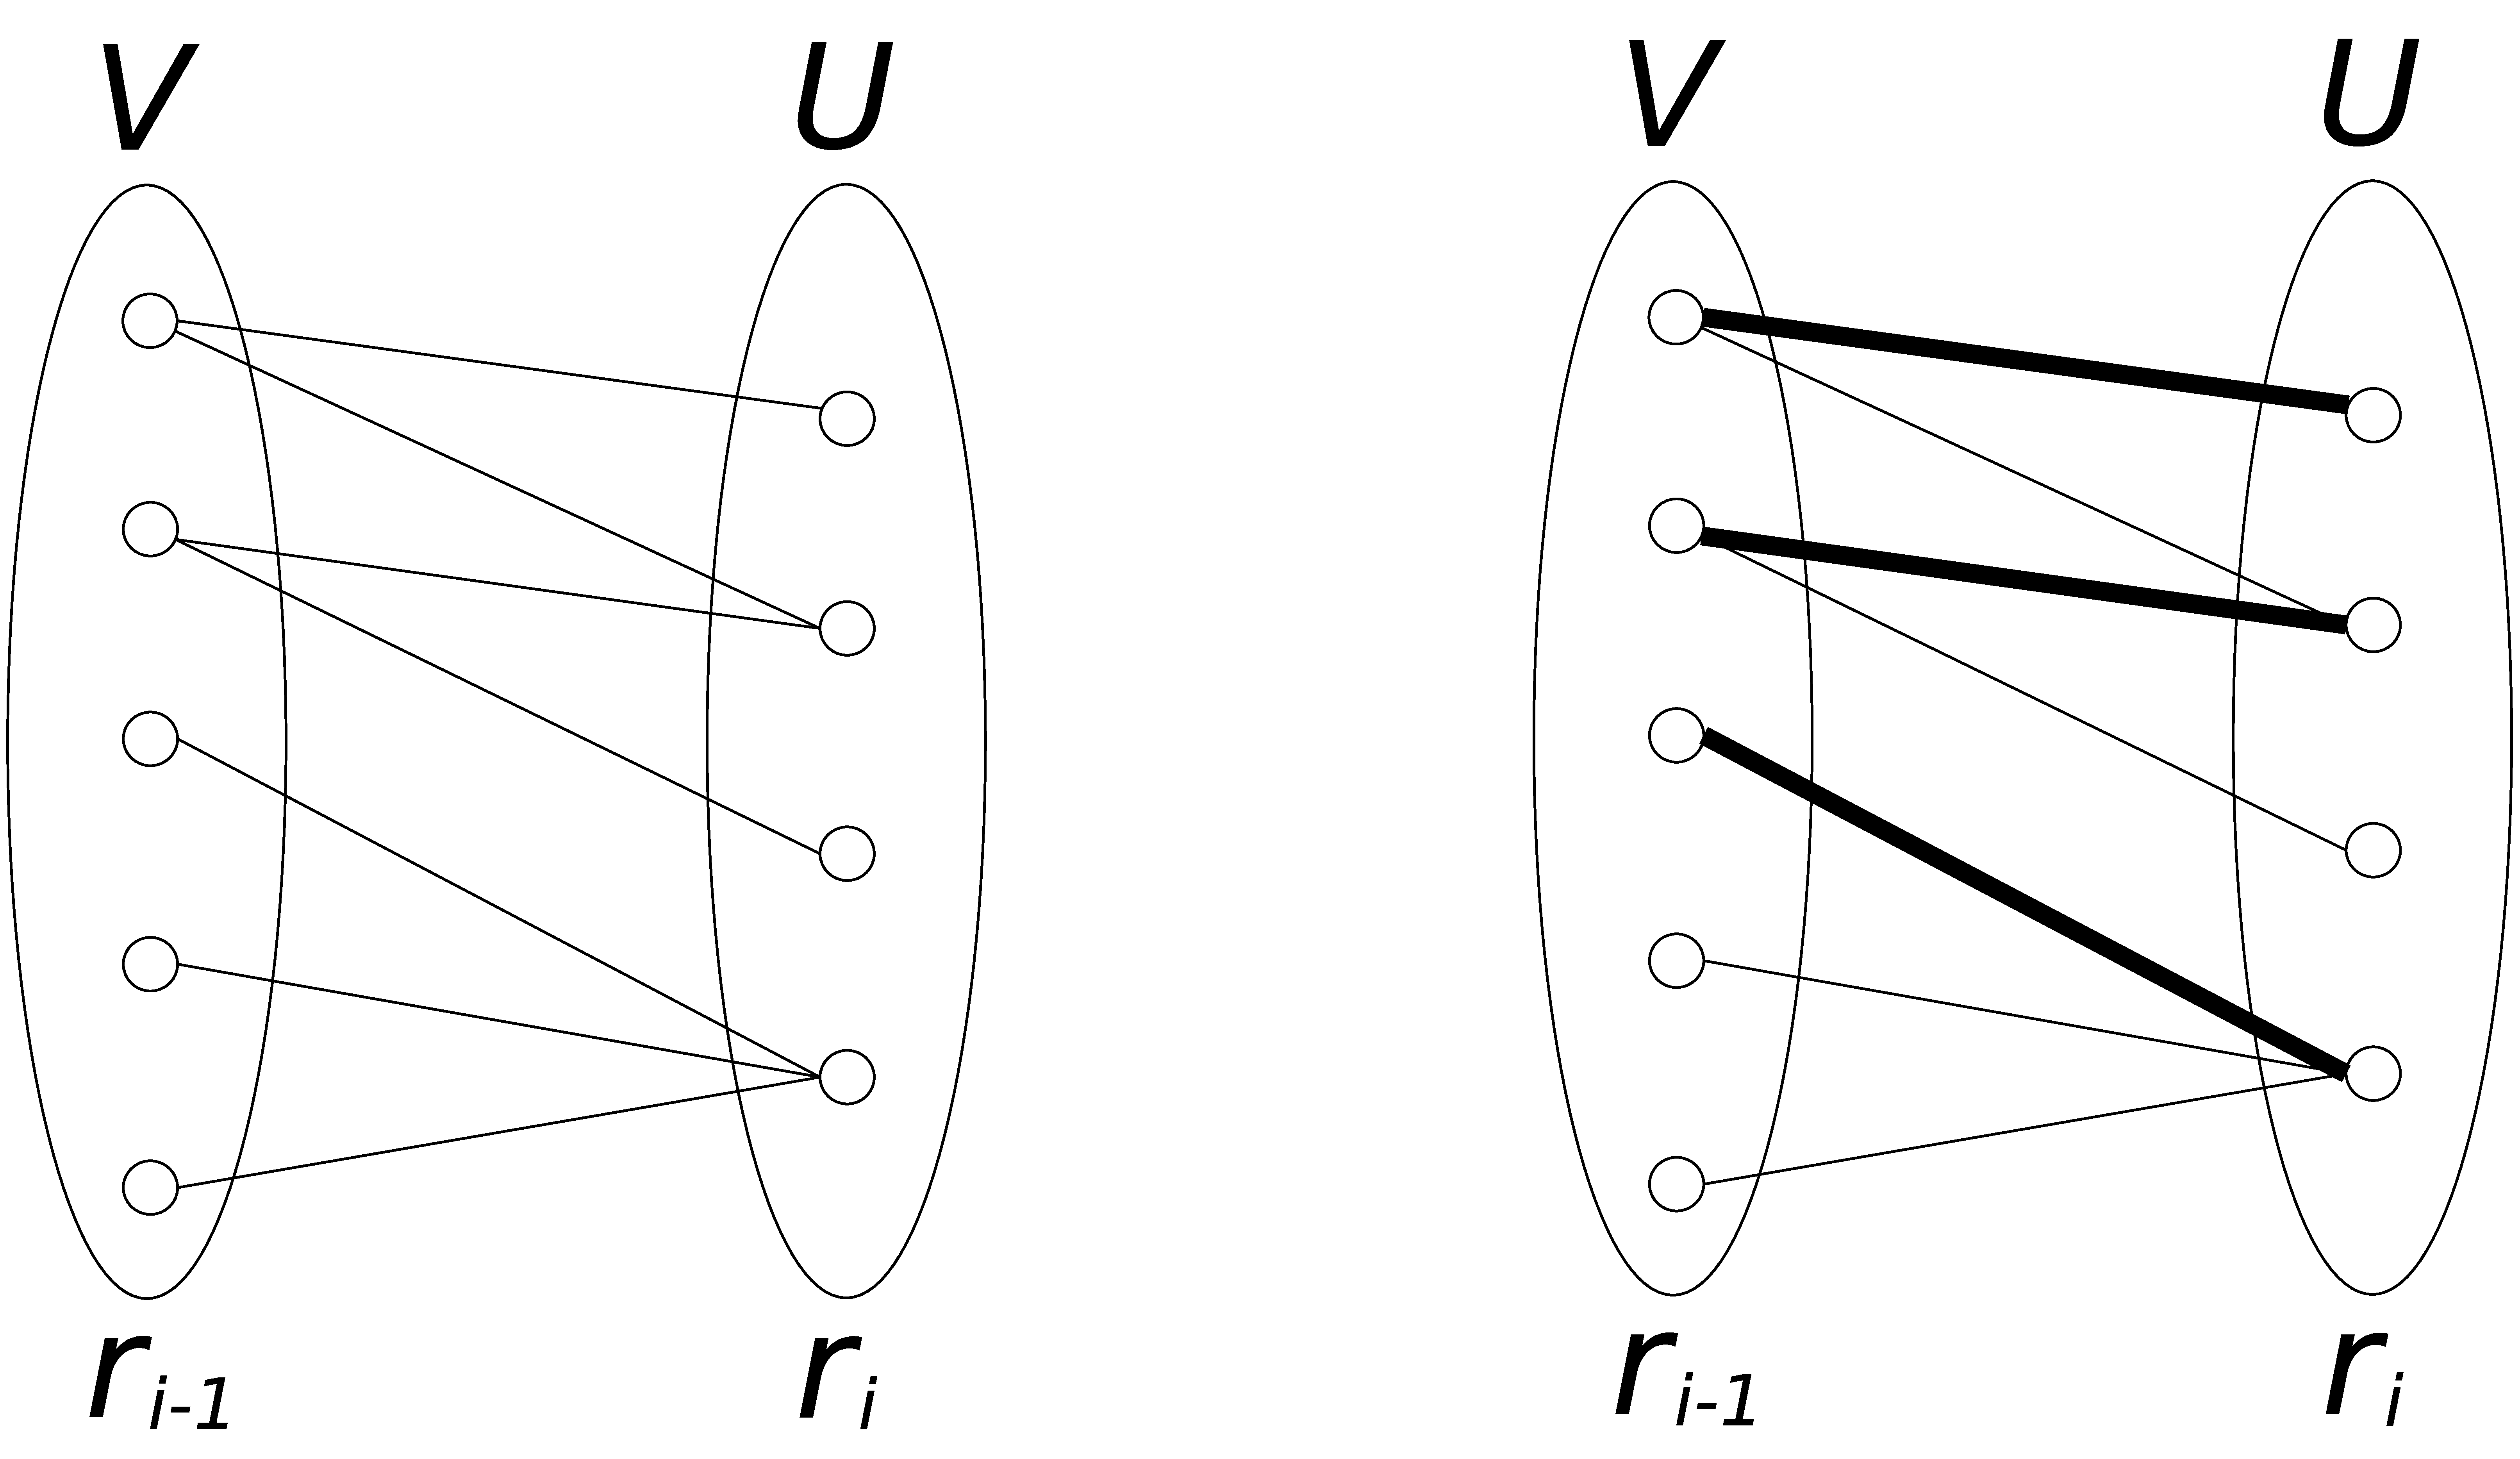
\includegraphics[height=4cm]{bipartite}
    \bicaption[fig:bigraph]{二分图}{一个二分图的例子和它其中一中匹配(被加粗的边)}{Bipartite Graph}{An example of bipartite graph and one of its matching (bold edges)}
\end{figure}
\begin{defn}[图的匹配]
    设$G(V,E)$是一个无向图,如果一个边集$M\subseteq E$中的边两两不相邻(即任意两条边不存在公共的顶点),则成$M$是$G$的一个匹配。
\end{defn}
图\ref{fig:bigraph}中的例子$G(U,V,E)$是一个典型的二分图。我们可以看到所有的边都横跨在两个点集$U,V$之间,而点集的内部不存在任何的边。
在二分图理论中最著名的问题莫过于“二分图最大匹配”问题\citen{west2001introduction},其旨在二分图$G(U,V,E)$中寻找一个最大的匹配$M$。
为了计算最大匹配的值$|M|$,我们需要引入组合数学中著名的霍尔定理\citen{hall1935representatives}的一个拓展:
\begin{thm}[霍尔定理\cite{hall1935representatives}的一个拓展]
    在一个二分图$G(U,V,E)$中,取$U$中的一个子集$X\subseteq U$,记$\Gamma(X)$为$X$的“邻居”,即所有$V$中与$X$中点相邻的点的集合。
    令$\delta(U)=max_{X\subseteq U}\{|X|-|\Gamma(X)|\}$,则有:
    $$MaxMatching(G)=|U|-\delta(U)$$
    \label{thm:hall}
\end{thm}
为了建立轮AKI问题与二分图之间的关系,我们需要这样思考:$r-1$轮和$r$轮的子密钥分别对应子集$V$和$U$中的一个顶点,而这两轮比特之间的一条依赖关系对应横跨$U,V$之间的一条边。
对于给定的子密钥集合$K$(均在$r$轮上),我们把$K$中所有的比特转化成顶点集合$U$,将$K$所依赖的所有$r-1$轮的比特转化为顶点集合$V$,他们之间的依赖关系转化为边集$E$,这样就可以构造出一张二分图$G(U,V,E)$。
这样构造之后,我们重新考虑定理\ref{thm:hall}中的子集$X$(可以视为$K$的一个子比特集合),它的“邻居”$\Gamma(X)$实际上包含了$X$依赖的所有$r-1$轮上的比特,即用$\Gamma(X)$中的所有比特可以推出$X$中的所有比特。
因此,我们可以得出以下引理:
\begin{lem}
    给定一个集中在一轮上的子密钥集合$K$和它的一个子集$X$,令$K'=\Gamma(X)\cup(K\backslash X)$,则$K'$是$K$的一个密钥信息集合。
\end{lem}
\begin{proof}
    由于$\Gamma(X)$可以推出$X$,而$K\backslash X$显然可以推出$K\backslash X$本身,则$K'$可以推出$K$,因此$K'$是$K$的一个密钥信息集合。
\end{proof}
为了找出$K$的实际密钥信息集合,我们需要找到一个最小的密钥信息集合。由于
$$|K'|=|K|-|X|+|\Gamma(X)|=|K|-(|X|-|\Gamma(X)|)$$
又由前文构造出的图$G(U,V,E)$,我们可以得到实际密钥信息集合$K'_{min}$必然满足:
\[
\begin{split}
    |K'_{min}|&=min\{|K|-|X|+|\Gamma(X)|\}\\
              &=|U|-max_{X\subseteq U}\{|X|-|\Gamma(X)|\}\\
              &=|U|-\delta(U)=MaxMatching(G) \qquad\ref{thm:hall}
\end{split}
\]
因此,一个子密钥集合$K$的实际密钥信息的值等于由$U=K$构造出的二分图$G(U,V,E)$的最大匹配的值,且实际密钥信息集合为$K'_{min}=\Gamma(X_{max})\cup(K\backslash X_{max})$,其中$X_{max}$是使$|X|-|\Gamma(X)|$最大的$X$。

\section{AKI-最小割算法}
上一章中提到的单轮加密的AKI只限于计算两轮之间的AKI值,无法将整个密码函数整体考虑。
黄佳琳博士在\citen{huang2014revisiting}中提到的AKI算法即为每次将密钥依赖路径中的一部分比特同时推至同一轮,考虑与同一轮比特之间的关系,这将会导致一些遗漏,下文将会提到其中的一个反例(该反例同样适用于Lin在\citen{lin2016automatic}提到的密钥桥算法)。
为了寻找一般情况下一个猜测集合的实际密钥信息集合,我们需要将单轮的特殊情况推向多轮的一般情况。
\subsection{一个简单的反例}
如果将猜测集合$K$中大于$r$轮的所有密钥都推到第$r$轮,同时考虑这些密钥与第$r$轮之间的依赖关系,使用上一节提到的二分图匹配算法寻找密钥信息集合,这将会遗漏一些特殊情况:
由于在这种情况下,密钥信息集合只可能取第$r$轮上的比特或是$K$中的比特,完全不考虑$r$轮之后的不在$K$中的比特,这很容易导致遗漏更小的密钥信息集合。
图\ref{fig:counter}提供了一个2轮密钥编排方案的反例,其中$K$为$r_2$轮上的3个比特。
在该反例中,无论是单独考虑$K$与$r_1$轮的密钥还是单独考虑$K$与$r_0$轮的密钥,都无法得出正确的实际密钥信息集合,因为真正的实际密钥信息集合中包含了分布在$r_0$和$r_1$两轮上的不同的比特。
因此,我们需要将所有轮密钥上涉及的比特统一考虑,才不会遗漏这种特殊情况。
\begin{figure}
    \centering
    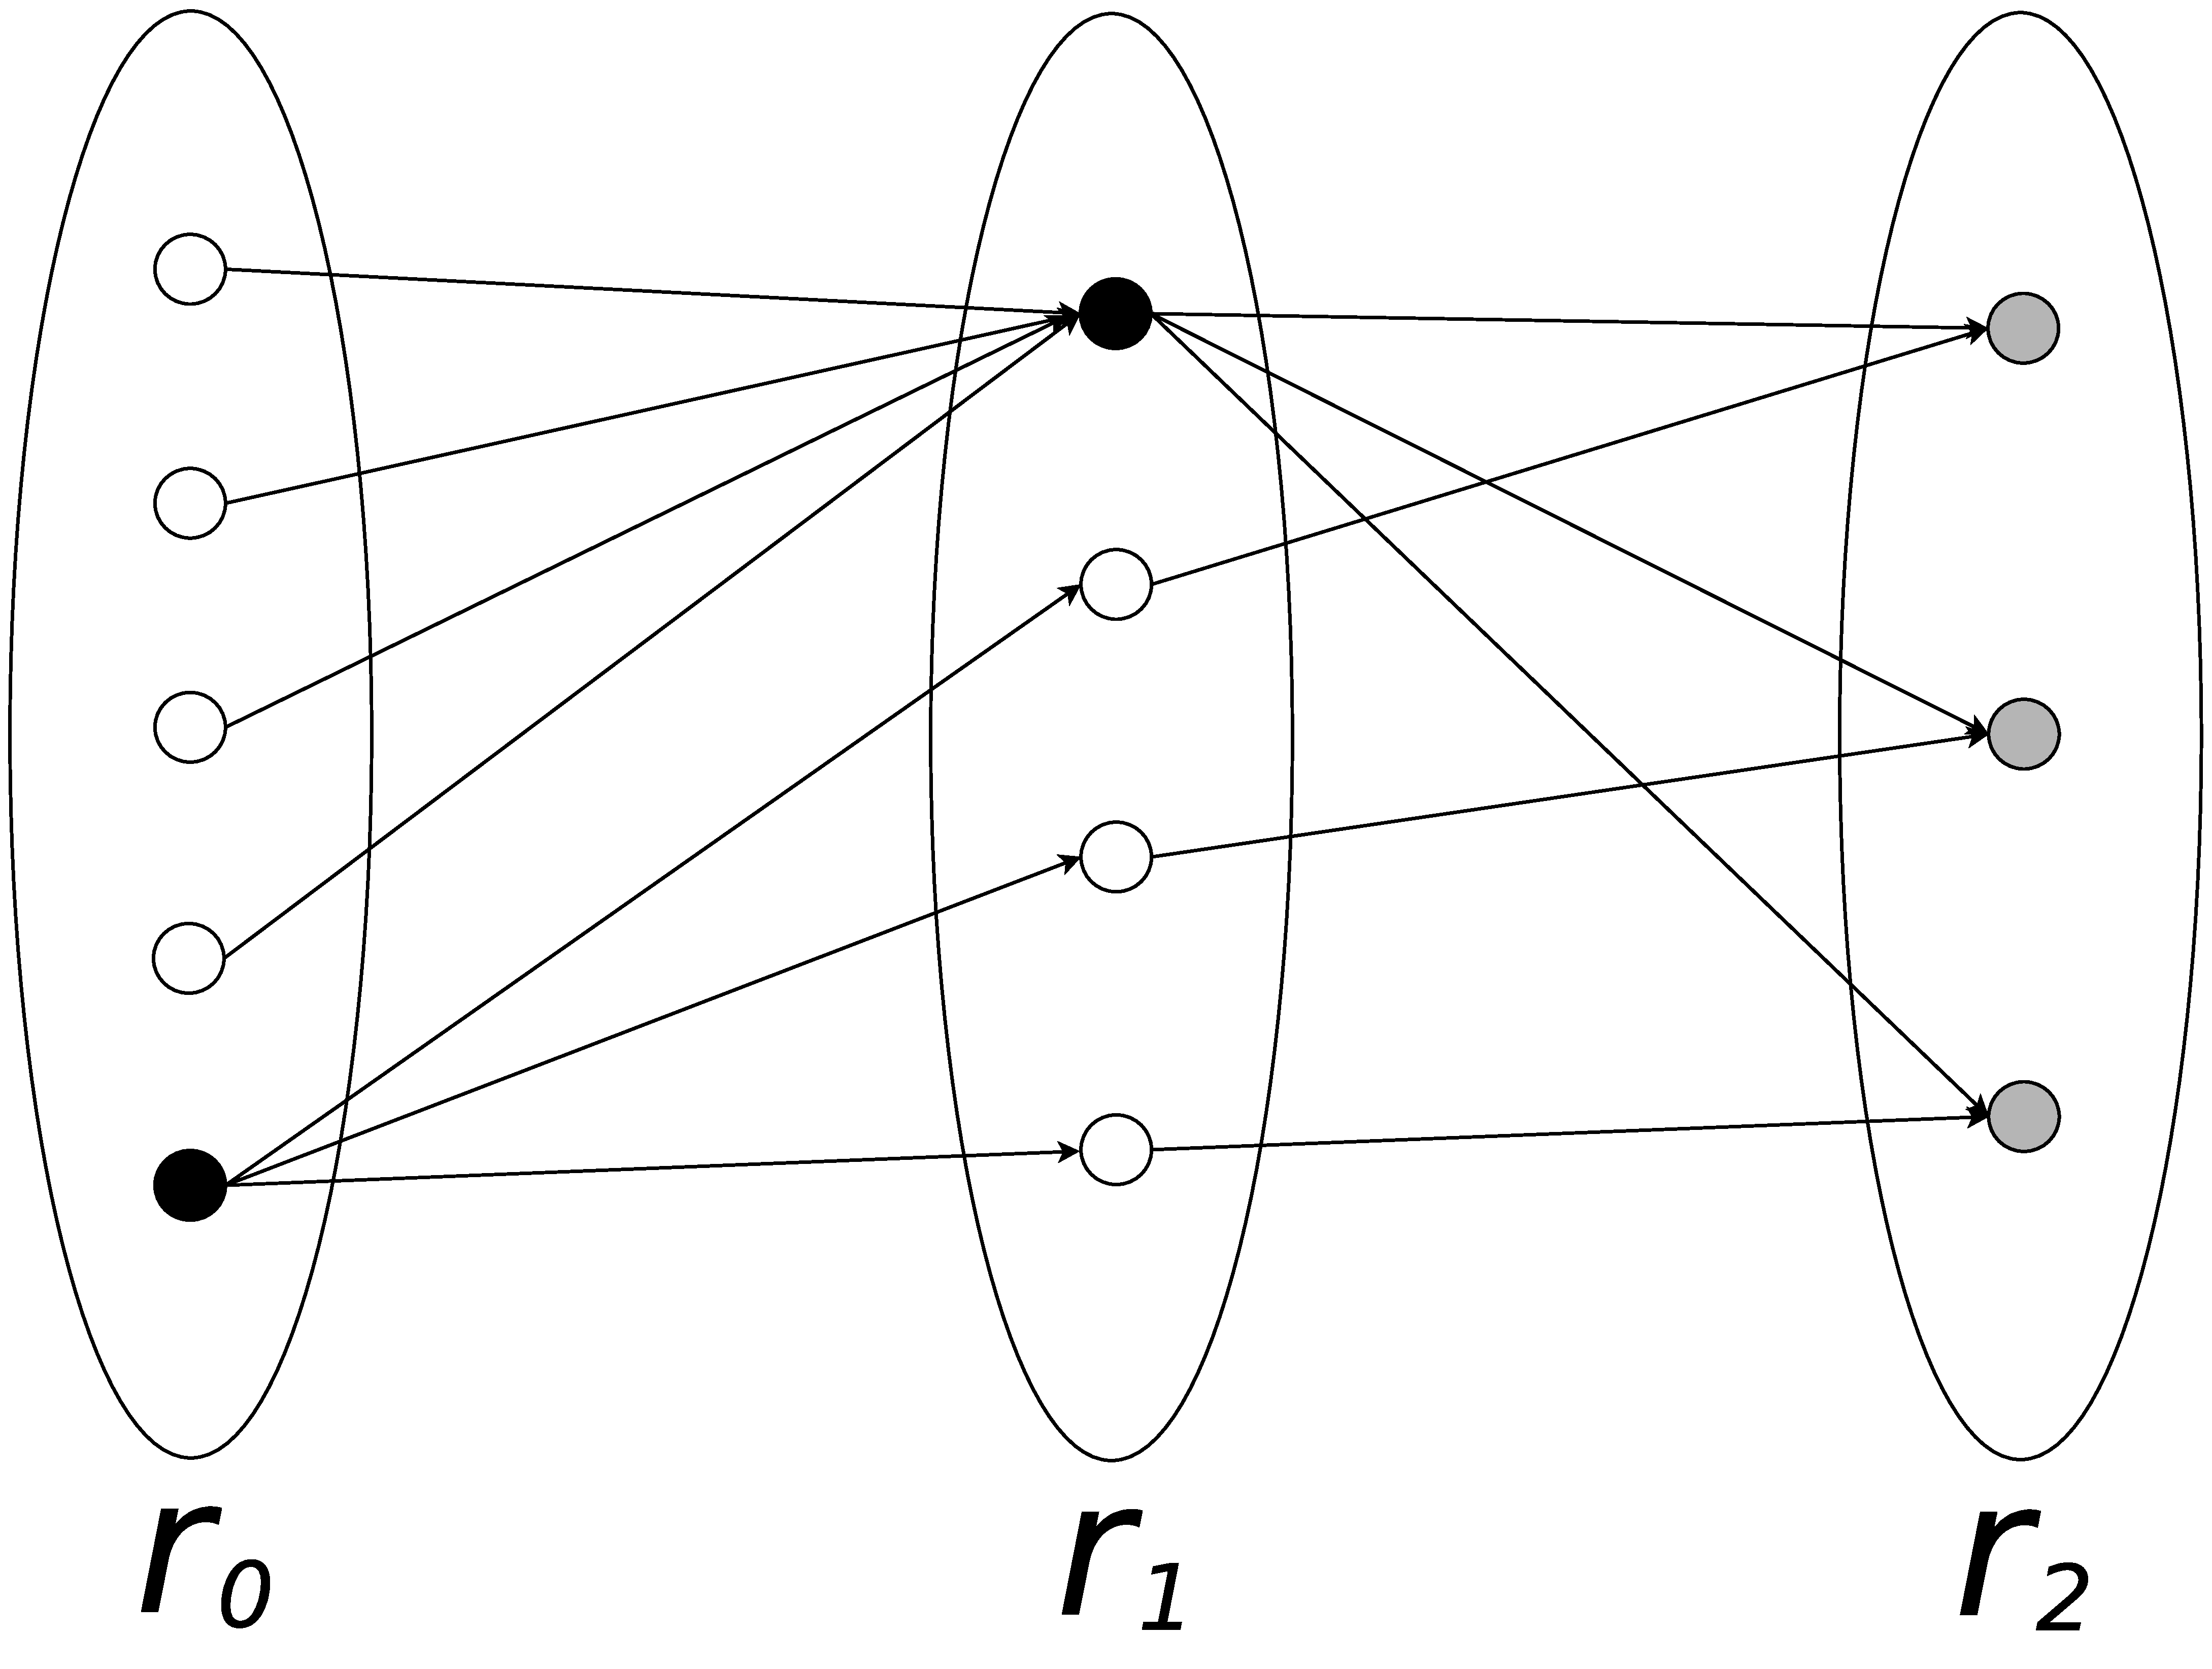
\includegraphics[height=3.3cm]{counter}
    \bicaption[fig:counter]{反例}{一个两轮密钥编排方案的反例,其中灰色的点代表猜测集合$K$,黑色的点是其实际蜜月信息集合。}{Counterexample}{The counterexample with a 2-round schedule. The bits in $K$ are filled with grey and the AKI-set bits are filled with black.}
\end{figure}
\subsection{最大流问题与最大流-最小割定理}
为了将所有轮密钥上的比特统一考虑,我们需要一个适用更加一般的情况的算法。
在图论中,二分图匹配问题是网络流最大流问题的一个特殊情况,因此我们猜想,真正的AKI算法将会使用网络流作为媒介来量化整个密钥编排方案。
在这一节中,我们将简单地介绍最大流问题以及最大流理论中非常重要的一个定理。
\begin{defn}[流量网络]
    一个连通的赋权有向图$G_f(V,E,c)$被成为一个流量网络(或容量网络),其中$c$是弧上的容量,并满足:
    \begin{enumerate}
        \item $c(u,v)$ 代表有向边$e=(u,v)$上的容量。如果$e\notin E$,则$c(u,v)=0$。
        \item 顶点集合中$V$有两个特殊的顶点$s$和$t$分别代表源点与汇点,并满足$\forall(u,v)\in E,u\neq t,v\neq s$(即不存在以t为起始或以s为终点的有向边)。
    \end{enumerate}
\end{defn}
\begin{defn}[流]
    一股流是一个对于所有顶点$u$和$v$都有以下特性的实数函数$f:V^2\rightarrow R$:
    \begin{enumerate}
        \item 容量限制(Capacity Constrains):$f(u,v)\leq c(u,v)$,即弧上的流不能超过该弧的容量;
        \item 斜对称(Skew Symmetry):$f(u,v)=-f(v,u)$,即由$u$到$v$的净流必须是由$v$到$u$净流的相反。
        \item 流守恒(Flow Conservation):除非$u=s$或$u=t$,否则$\sum_{v\in V}f(u,v)=0$,即除了源点与汇点以外的所有点流出的流量为0。
    \end{enumerate}
    流$f$的大小定义为$val(f)=\sum_{u\in V}f(s,u)$。
\end{defn}
最大流问题旨在流量网络$G_f(V,E,c)$中寻找一个最大的流$f$。目前有很多解决该问题的算法,例如Ford-Fulkerson算法\citen{ford1956maximal},预留推进算法,Dinic算法\citen{dinits1970algorithms}等。

最大流问题的对偶问题——最小割问题,同样是十分著名的图论问题之一。
\begin{defn}[割]
    设$S$和$T$为流量网络$G_f(V,E,c)$顶点集合$V$的一个分割,即$S\cup T=V$且$S\cap T=\varnothing$,并满足$s\in S,t\in T$,则称$C=(S,T)$为流量网络$G_f$的一个割。
    其中割$C(S,T)$的大小定义为:
    $$cap(C)=\sum_{(u,v)\in E,u\in S,v\in T}c(u,v),$$
    即为$G_f$中所有从$S$到$T$的弧的容量总和。
\end{defn}
\begin{figure}[htbp]
\centering
    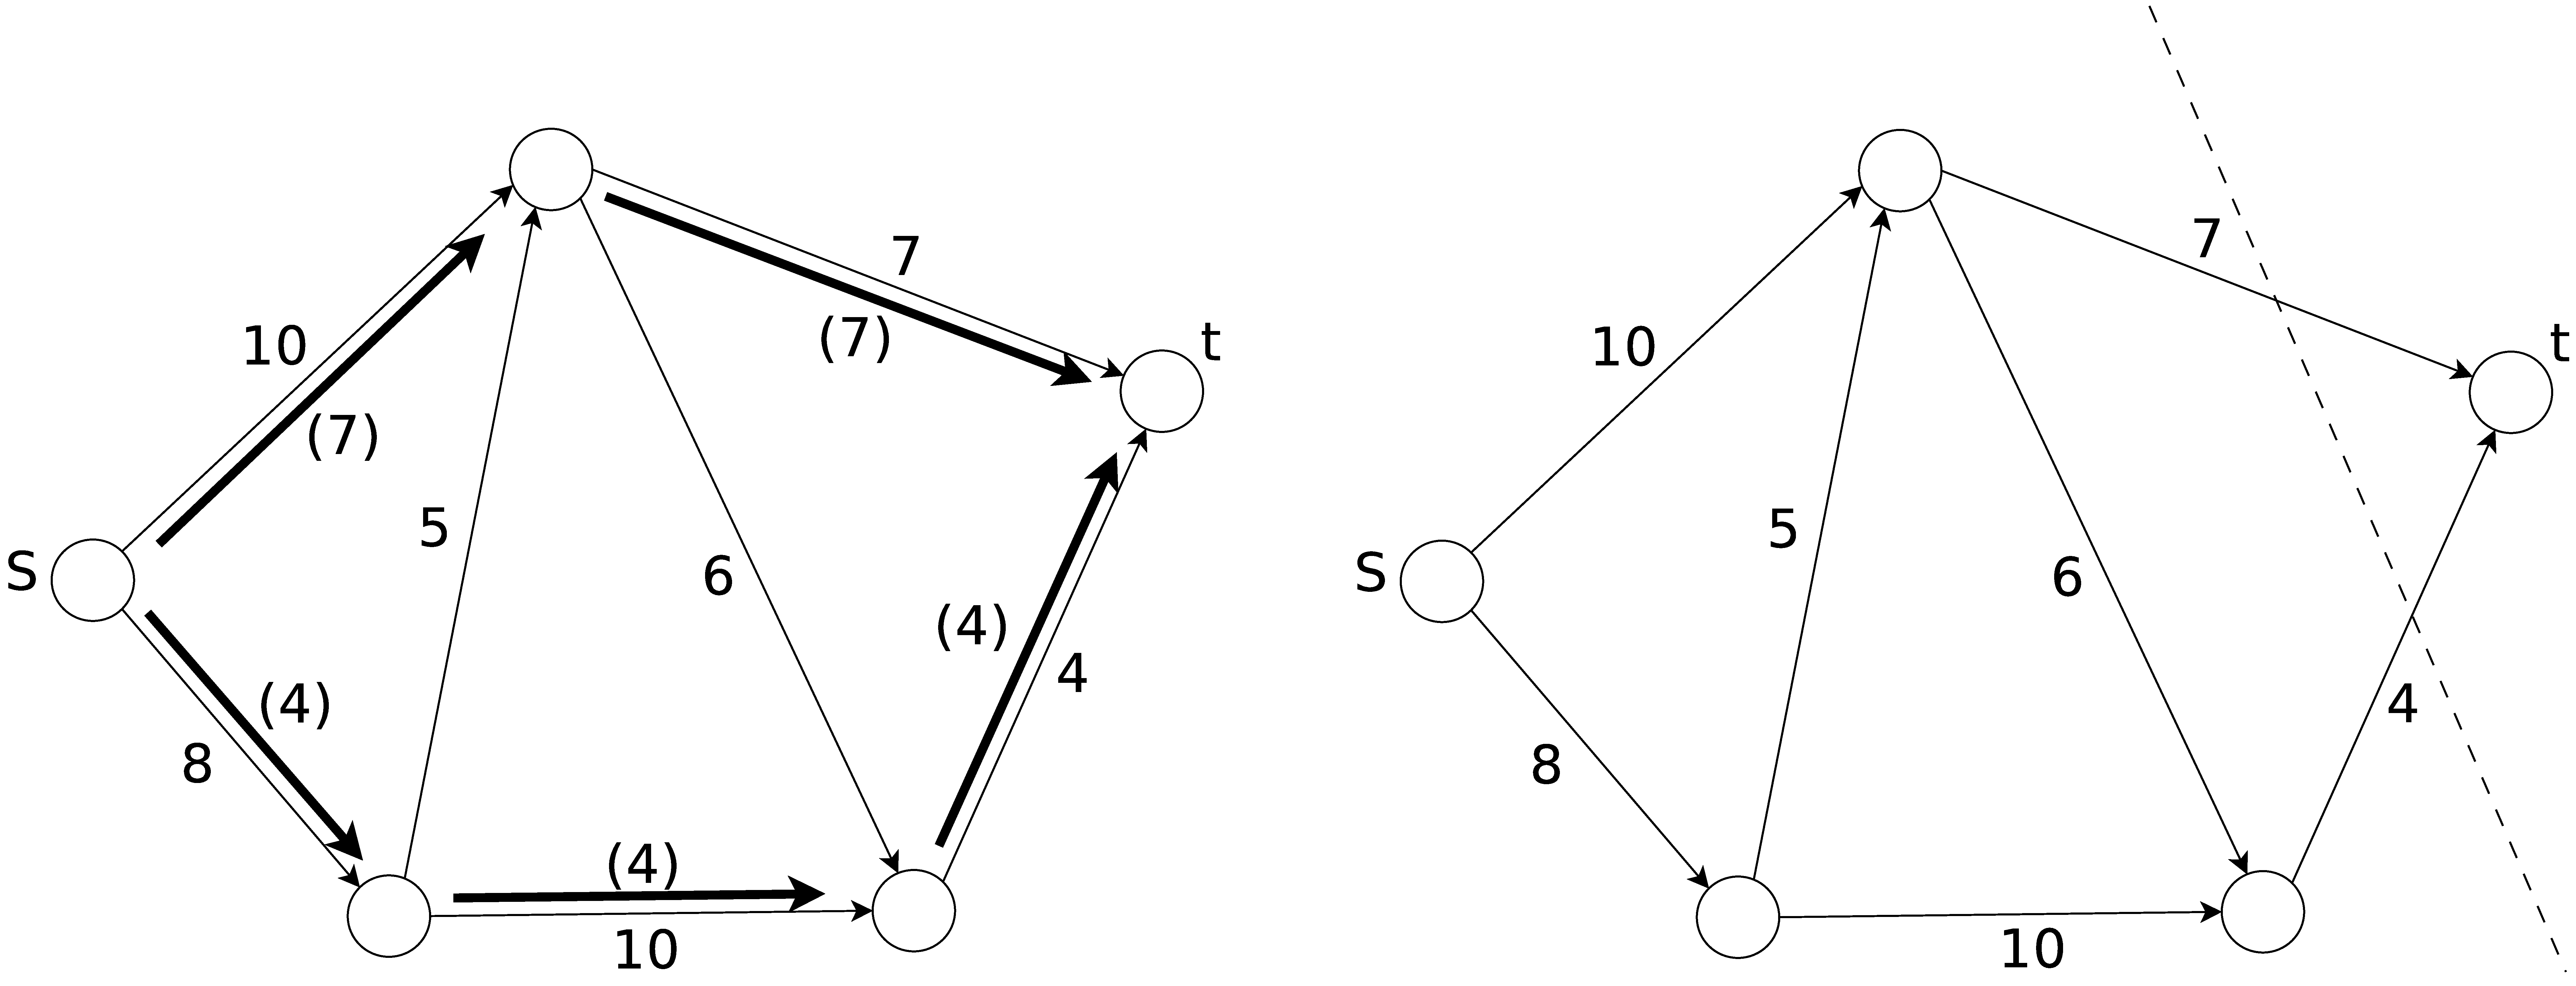
\includegraphics[height=4.5cm]{flowcut}
    \bicaption[fig:flowcut]{最大流与最小割}{一个流量网络的样例中的最大流(左图加粗的边和括号中的数字)和最小割(右图的虚线)}{Max-flow and Min-cut}{An exmaple flow network with its capacities and one of its max-flow (the bold edges and enclosed numbers) and its min-cut (the dotted line)}
\end{figure}
而最大流问题与最小割问题的对偶关系可以由网络流理论中著名的最大流-最小割定理来说明:
\begin{thm}[最大流-最小割定理\citen{papadimitriou19986}]
    在一个流量网络$G_f(V,E,c)$中,最大流的大小等于最小割的大小。
\end{thm}

\section{算法描述}
通过上一节关于最大流与最小割问题的介绍,我们大致了解了最大流与最小割的含义与性质。
在这一节中,我们将介绍一个全新的基于最大流最小割理论的AKI算法——AKI-最小割算法。
该算法旨在将密钥编排方案(用其密钥依赖矩阵$M$表示)和猜测集合$K$转化为一个流量网络$G_f(E,V,c)$,然后在该网络上求最小割来寻找实际蜜月信息集合。

为了建立
